\documentclass[a4paper,11pt]{article}

\usepackage[utf8]{inputenc}
\usepackage[T1]{fontenc}
\usepackage{lmodern}
\usepackage{graphicx}
\usepackage{makeidx}
\usepackage{index}
\usepackage{url}
\usepackage{float}
\usepackage[dvipsnames,usenames]{color}
\usepackage{xcolor}
\usepackage{listings}
%\usepackage[frenchb]{babel}

\lstloadlanguages{C++}
\lstset{
    keywordstyle=\tt\bf,
    identifierstyle=\tt,
    commentstyle=\tt\color[rgb]{0.133,0.545,0.133},
    stringstyle=\tt\color[rgb]{0.627,0.126,0.941},
    showstringspaces=false,
    basicstyle=\footnotesize,
    numberstyle=\footnotesize,
    numbers=left,
    stepnumber=1,
    tabsize=2,
    breaklines=true,
    breakatwhitespace=false,
    columns=fixed,
    extendedchars=true,
}

% Informations sur le document.
\title{Rapport Final - PAPPL} \author{Clément \textsc{Delafargue}\\Benjamin \textsc{Vialle}} \date{\today}

% Indentation sur le premier paragraphe d'un chapitre ou section.
%\usepackage{indentfirst}

% Réglage des marges
\usepackage{geometry}
\geometry{left=2cm, right=2cm, top=2.5cm, bottom=2.5cm}

% Mise en forme des en-têtes et pieds de page.
\usepackage{fancyhdr}
\pagestyle{fancy}
\setlength{\headheight}{1.5cm}
\setlength{\textheight}{23cm}
\setlength{\footskip}{2cm}
\lhead{Final Report - PAPPL}
\rhead{\leftmark}
\lfoot{
\includegraphics[height=1.5cm]{images/ECN.pdf}}
\rfoot{
\includegraphics[height=1.5cm]{images/OOo4Kids.png}}
\fancyfoot[C]{}
\renewcommand{\headrulewidth}{0.4pt}
\renewcommand{\footrulewidth}{0.4pt}

% PDF hyper-linking (set colors to black for printing)
\usepackage[colorlinks]{hyperref}
\usepackage[figure,table]{hypcap}
\hypersetup{
	bookmarksnumbered,
	pdfstartview={FitH},
	citecolor={blue},
	linkcolor={black},
	urlcolor={black},
	pdfpagemode={UseOutlines}
}
\makeatletter
\newcommand\org@hypertarget{}
\let\org@hypertarget\hypertarget
\renewcommand\hypertarget[2]{%
  \Hy@raisedlink{\org@hypertarget{#1}{}}#2%
} 
\makeatother 

%Pour les sauts de ligne entre les paragraphes
\setlength{\parskip}{6pt}

%Supprimer l'alinea
\parindent=0pt

%Pour l'index à la fin du rapport
\makeindex

% Début du document.
\begin{document}

% Définition de la page de garde.
	\begin{titlepage}

		% Pas d'en-tête et pied de page ni de numérotation de page.
		\thispagestyle{empty}

		% Logo Centrale
		\begin{flushleft}
			
\includegraphics[scale=0.8]{images/ECN.pdf}
		\end{flushleft}

		\vfill
		
		\begin{center}
			{\Large \textsc{École Centrale de Nantes}} \\

		\vspace{1cm}

		%Insertion d'un titre entouré de traits horizontaux.
		\begin{tabular}{p{0cm} c}
			\hline
			& \\
			& {\huge {\bfseries Final Report - PAPPL}} \\
			& \\
			\hline
		\end{tabular}

		\vspace{2.5cm}

		\texttt{{\large Application Project - OpenOffice.org4Kids}} \\
		\texttt{{\large January, 2011 - March 2011}} \\

		\vspace{2.5cm}

		% Insertion de deux noms		
		\begin{tabular}{l c r}
			\large{\emph{Author:}} & \hspace{5cm} & \large{\emph{Supervisor:}} \\
			\large{Clément \textsc{Delafargue}} & \hspace{5cm} & \large{Éric \textsc{Bachard}}\\
			\large{Benjamin \textsc{Vialle}} & \hspace{5cm} & \large{Morgan \textsc{Magnin}}\\
		\end{tabular}

		\end{center}

		\vfill

		% Insertion logo Rails
		%\begin{flushleft}
		%	\includegraphics[scale=0.3]{Ruby_on_Rails_logo.jpg}
		%\end{flushleft}
		
		\begin{tabular}{l c r}
				 
\includegraphics[scale=0.4]{images/logo_EducOOo.jpg}  & \hspace{6cm} & 
\includegraphics[scale=0.4]{images/OOo4Kids.png}  \\
		\end{tabular}
		
		% Insertion logo MarkUs
		%\begin{flushright}
		%	\includegraphics[scale=2]{markus.png}
		%\end{flushright}
		
	\end{titlepage}


\newpage
\tableofcontents
% Il faut compiler plusieurs fois pour obtenir une table des matière correcte.

\newpage

% Introduction sur une page, section non numérotée et intégrée à la table des matières.
\setcounter{page}{1}
\rhead{\Large{\textsc{Thanks}}}
\fancyfoot[C]{\thepage}
\section*{Thanks}
\addcontentsline{toc}{section}{Thanks}
A particular thanks to Éric \textsc{Bachard}, our mentor during this project. He helped us and was always available on IRC.

Thanks to Nelle \textsc{Varoquaux}, for her code reviews on our patches and help.

Thanks to our teacher, Morgan \textsc{Magnin}.

\newpage

\rhead{\Large{\textsc{Introduction}}}
\fancyfoot[C]{\thepage}
\section*{Introduction}
\addcontentsline{toc}{section}{Introduction}

\subsection*{Context}
\addcontentsline{toc}{subsection}{Context}

Several groups of Centrale Nantes have worked on enhancing the User eXperience
of OpenOffice.org on TabletPCs. In particular they have worked on the
annotation module of Impress: when in slideshow mode, the user is able to
annotate the slides by drawing shapes with the mouse. It is also possible to
remove parts of these shapes with an eraser tool.

Our work aimed at prolonging this work by:

\begin{itemize}

\item reading their reports\footnote{Some parts of their reports were re-used
here, because they were very similar.};

\item correcting the last of their bugs;

\item implementing new relevant functionalities in OpenOffice.org Impress in
prolongation of their work.

\end{itemize}

In september 2010, OpenOffice.org was forked. A lot of developpers went to
LibreOffice. Éric \textsc{Bachard} stays working with his team on
OpenOffice.org4Kids (OOo4Kids). They are not related to LibreOffice.

\paragraph{Useful acquired knowledge for the continuation of the project} : we
learned to handle the code of modules around OpenOffice.org Impress as well as
C++, what was not intuitive because we were more developers been used to Java.
Éric Bachard tought us how to compile and the basis of OpenOffice.org4Kids
development (rudiments on the conventions of naming C++, how files were
organized in OOo4Kids tree). And we finally learnt to communicate in a simple
and fluid way with the developers of OpenOffice.org4Kids, via the channel
\url{educooo} and \url{ooo4kids} on \url{irc.freenode.net}.

\subsection*{Organization}
\addcontentsline{toc}{subsection}{Organization}

The work was divided the following way:
\begin{itemize}
\item Clément was Developper and handled the compilation on his computer
(which is way faster than Benjamin's one)
\item Benjamin was Developper and responsible of communication with Éric \textsc{Bachard}
\end{itemize}

We both maintained pages on OpenOffice4Kids' wiki :
\url{http://wiki.ooo4kids.org/index.php/User:Bvialle} and
\url{http://wiki.ooo4kids.org/index.php/User:Clementd}

\newpage

\rhead{\Large{\textsc{Project requirements}}}
\fancyfoot[C]{\thepage}
\section*{Project requirements}
\addcontentsline{toc}{section}{Project requirements}

\subsection*{Specifications}
\addcontentsline{toc}{subsection}{Specifications}


\subsubsection*{Project overview}
\addcontentsline{toc}{subsubsection}{Project overview}

OpenOffice.org For Kids is a lightweight version of OpenOffice.org
specifically designed for an educational use.

Students of Centrale Nantes have already contributed to OOo4Kids in the past,
namely on the annotation feature in Impress, in order to enhance the
integration with Tablet PCs.


\subsubsection*{Annotation feature}
\addcontentsline{toc}{subsubsection}{Annotation feature}


\paragraph*{Layout of the presenter screen} :

We have to understand how the overlay works : how eraser and pen have been
added to the layout. We also have to understand how UNO works.



\paragraph*{Source code cleanup}

Some source files are not cleanly organized and formatted. While developing
the features, we will clean those files (properly indent the code, delete
trailing spaces, regroup the lines correctly).


\paragraph*{Drawing modes}

When enabling the annotation feature, the user is in the \emph{cursor} mode,
and then can switch to the \emph{pencil} mode or the \emph{eraser} mode. When
in \emph{pencil} or \emph{eraser} mode, it is tedious to go back to the cursor
mode. A first task would be to allow the user to go back to the \emph{cursor}
mode.

The main part of the code is located in
\emph{slideshow/source/engine/slide/slideshowimpl.cxx}.

\begin{figure}[!h]
\centering
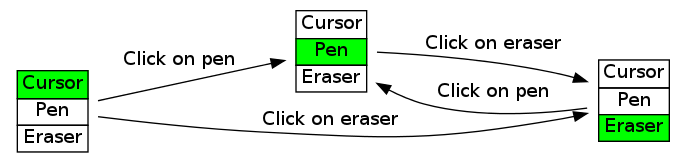
\includegraphics[scale=0.5]{images/modes_current.png}
\caption{Current mode switching}
\end{figure}

\begin{figure}[!h]
\centering
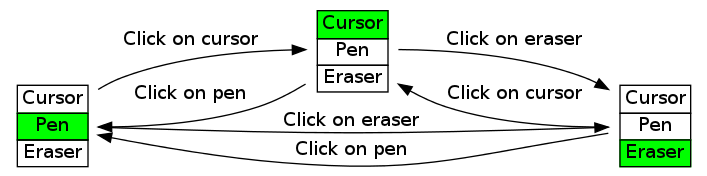
\includegraphics[scale=0.5]{images/modes.png}
\caption{A better mode switching}
\end{figure}

We will have to add a new menu entry (\emph{cursor}), in order to allow the
user to easily go back to the cursor mode. This will require us to change the
underlying structure of some files.

\paragraph*{Eraser}

When in the eraser mode, the tool only masks parts of the previously drawn
shapes. It does not actually delete the erased parts. In addition, nothing is
saved. When leaving the slide, then displaying it again, the erased parts
reappear.

Erased parts should be really erased and not displayed again when displaying
the slides.

The team is looking forward to implementing a do/undo feature in the
annotation mode (while presenting the slides), but nothing is decided now.

\subsubsection*{Products}
\addcontentsline{toc}{subsubsection}{Products}

\begin{itemize}
\item OpenOffice.org4Kids patch, containing our contribution;
\item documentation on the project (setup, project progress, code documentation).
\item weekly article on OpenOffice.org4Kids' wiki.
\end{itemize}


\subsubsection*{Product approval criteria}
\addcontentsline{toc}{subsubsection}{Product approval criteria}

The code must be  \textbf{OpenOffice.org normalized}, compile correctly, be
documented and tested. Éric \textsc{Bachard} will test every patch.

\newpage

\rhead{\Large{\textsc{Project contents and achievements}}}
\fancyfoot[C]{\thepage}
\section*{Project contents and achievements}
\addcontentsline{toc}{section}{Project contents and achievements}

\subsection*{Technical aspects}
\addcontentsline{toc}{subsection}{Technical aspects}

\subsubsection*{Setting up a development environment}
\addcontentsline{toc}{subsubsection}{Setting up a development environment}


Our first difficulty was to set up a development environment . The OOo4Kids is
hosted on SVN\footnote{\url{svn://svn.adullact.net/svnroot/ooo4kids1/trunk}}.

We decided to use Git to work with our own branches and to be independant from
svn. We wanted to work separately and be able to synchronize our repositories.
We clone and did a fork of OOo4Kids' svn. They were hosted on the
\emph{serveur des élèves} in Centrale
Nantes\footnote{\url{gitosis@campus.ec-nantes.fr:o4k-divarvel.git} and
\url{gitosis@campus.ec-nantes.fr:o4k-benjaminvialle.git}}.  Cloning the code
took us about 1 hour (12,4 Gb, and more of 200 000 items to download).
   
\begin{figure}[!h]
\centering
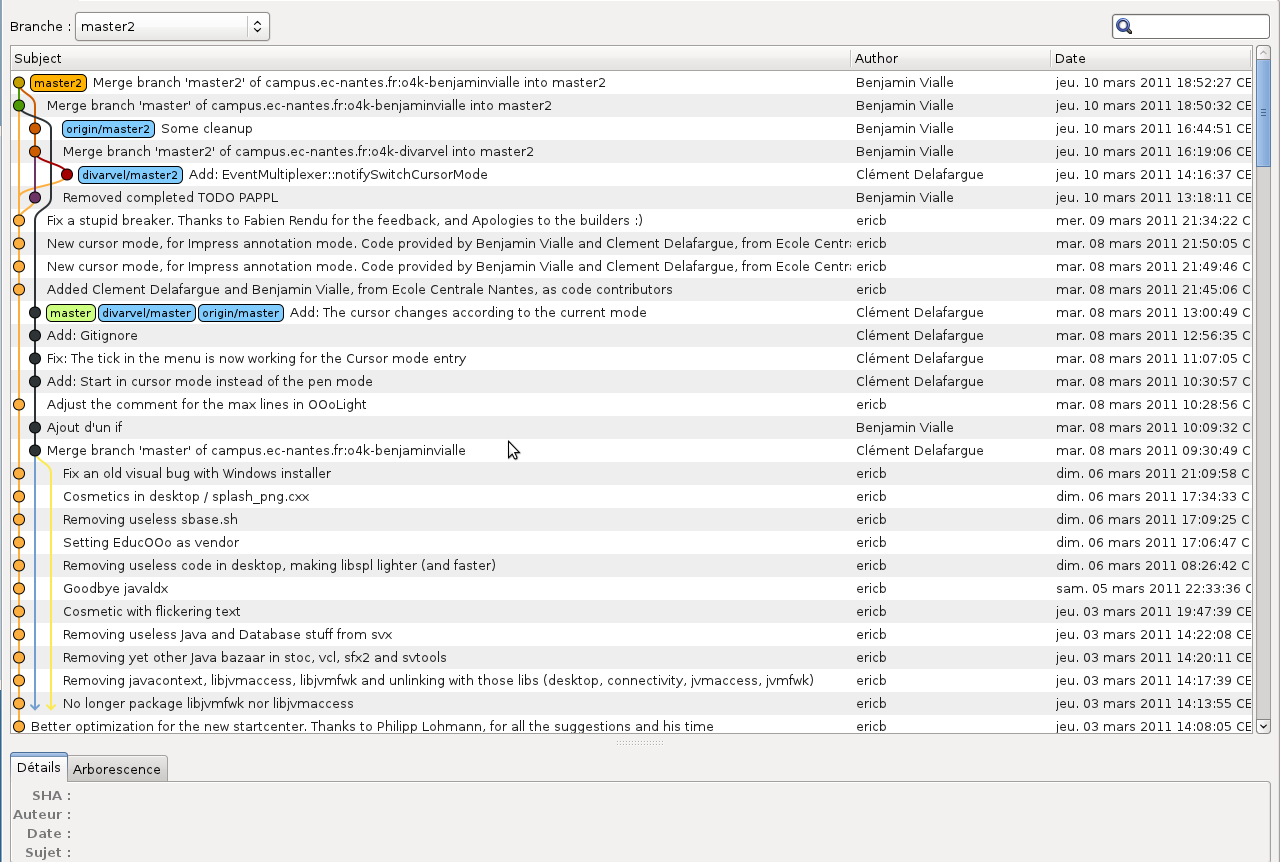
\includegraphics[scale=0.3]{images/Gitg.png}
\caption{Branching is easy with Git}
\end{figure}   
   
Compiling was another problem. The two computers we were using were working on
GNU/Linux, one with Gentoo and the other with Ubuntu.

On the Jaunty computer, we just followed the OpenOffice.org tutorial2 . When
we tried to run the configure script, we faced several errors. By studying
them, we were able to install most of the missing packages. Once the configure
ran properly, the build happened without any error !

On the Ubuntu computer, after doing exactly the same thing, the configure
script ran properly and the build was a success.

Since we had so many difficulties, we wrote down a tutorial for
Gentoo\footnote{see
\url{http://wiki.ooo4kids.org/index.php/EnvironmentSetup/Linux\#Build\_and\_install\_on\_Gentoo\_Linux}}.

Moreover, we discovered a bug on OpenOffice.org compilation on Gentoo\footnote{see
\url{http://wiki.ooo4kids.org/index.php/User:Bvialle\#Husnpell\_issues}}.
According to Éric, this bug appears also on *BSD systems. And clearly, Gentoo
as a lot of things in common with *BSD systems, in particular their way to
build packages. Portage, Gentoo's package manager is inspired of port, *BDS
package manager. They are both retrieving dependencies and compiling them ! It
was the first time we built OpenOffice.org4Kids on a Gentoo system.

Once the first build was complete, we could shorten the time spent compiling,
by building only the module that had been changed. Once again, the
documentation we found was incomplete and hard to apply. Éric \textsc{Bachard}
help us a lot improving compilation.

Moreover, Benjamin's abilities on Gentoo made him the possibility to built a
very fast environment using \emph{ccache} and \emph{distcc}. Ccache is a cache
for C and C++. The compiler use it as many times as possible to speed up the
compilation phase. Distcc is a way to share compilation times between
computers. We did it with Benjamin's UC (a Quad Core with 4GB of RAM).


\subsubsection*{Architecture and Design}
\addcontentsline{toc}{subsubsection}{Architecture and Design}

OpenOffice.org’s (and OpenOffice.org4Kids) code is organized in modules. Thanks to
PGROU-2008’s report, we immediately knew only two modules interested us, the
slideshow module, and the sd module, containing the User Interface. Next
picture allows to understand how OpenOffice.org works from the User Interface to
spread all the modifications.

\begin{figure}[!h]
\centering
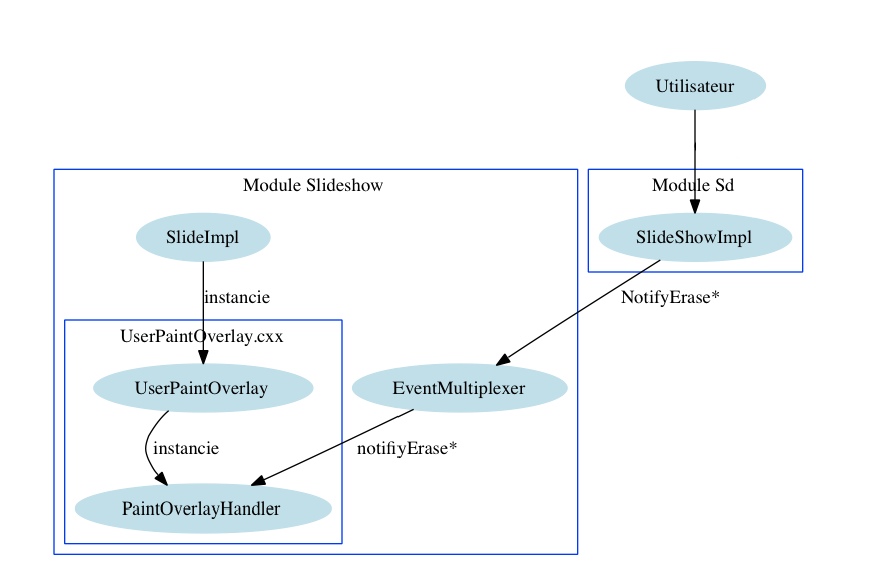
\includegraphics[scale=0.5]{images/Slideshow_interaction.png}
\caption{How classes and objects intercats in OOo4Kids}
\end{figure}   

\paragraph*{Inside the sd module}
The sd module contains all the code concerning the implementation of the
contextual menu. If we go through the path \emph{sd/source/ui/slideshow}, we
can observe different types of file.

\textbf{localize.sdf}

\begin{verbatim}
sd source/ui/slideshow/slideshow.src                0 menuitem
RID_SLIDESHOW_CONTEXTMENU CM_ENDSHOW                0 ar 2002-02-02 02:02:02
sd source/ui/slideshow/slideshow.src                0 menuitem
RID_SLIDESHOW_CONTEXTMENU CM_ENDSHOW                13691 as-IN 2002-02-02 02:02:02
\end{verbatim}

This file contains all the internationalization of the text contained in the
menu. This part is only modified by Sun developers.

\paragraph*{slideshow.src} Contains the skeleton of the menu. Each item of the
menu is written, in the order it should appear. Each one has an identifier.
So, first step, we could add our menu item for the \emph{Cursor Mode}. We both
added an entry for english and french.

\begin{verbatim}
 77ifdef ENABLE_PRESENTER_EXTRA_UI
 78         MenuItem
 79         {
 80             Identifier = CM_CURSOR_MODE;
 81             Text [ en-US ] = "~Cursor Mode";
 82             Text [ fr ] = "~Curseur";
 83         };
 84         MenuItem
 85         {
 86             Identifier = CM_PEN_MODE;
 87             Text [ en-US ] = "~Pen Mode";
 88         };
 89         MenuItem
 90         {
 91             Identifier = CM_ERASE_MODE;
 92             Text [ en-US ] = "~Eraser Mode";
 93         };
 94         MenuItem
 95         {
 96             Separator = TRUE;
 97         };
\end{verbatim}

    There are different possible types of element: a link, a submenu, a
separator etc... Menu, submenu and links must have and identifier. This
identifier must be declared in the header of this file, \emph{slideshow.hrc}.

\begin{verbatim}
64 #define CM_CURSOR_MODE 29
\end{verbatim}

To each identifier is associatied a number, which needs to be unique.

\paragraph*{slideshowimpl.cxx and slideshowimpl.hxx}

This file is used to enable or disable items, and to add checkbox to them in
the menu. This way, you can disable an action that has no sens of being in the
menu:

\begin{lstlisting}[language=C++]
#ifdef ENABLE_PRESENTER_EXTRA_UI
	//adding button to contextual menu for erasing functionnalities
	// for UserPaintOverlay
	pMenu->EnableItem( CM_ERASE_ALLINK, (maPresSettings.mbMouseAsPen));
	// Adding button to contextual menu for changing pen color
	pMenu->EnableItem( CM_COLOR_PEN, (maPresSettings.mbMouseAsPen));
	// Adding button to display if in Cursor mode
	pMenu->EnableItem( CM_CURSOR_MODE, (maPresSettings.mbMouseAsPen));
	// Adding button to display if in Pen  mode
	pMenu->EnableItem( CM_PEN_MODE, (maPresSettings.mbMouseAsPen));
	// Adding button to display if in Erase Mode
	pMenu->EnableItem( CM_ERASE_MODE, (maPresSettings.mbMouseAsPen));
#endif
\end{lstlisting}

For example, the menuItem CM\_CURSOR\_MODE, corresponding to the link "Next",
is visible only if there is a slide after the one we are currently on.  In
this file are also all the actions that follow the selection of one action. It
can be a hover on a link to a submenu, a click on a link to an action, or key
pressed. Depending on the identifier, it will call a method, in this same
class:

\begin{lstlisting}[language=C++]
            case CM_CURSOR_MODE:
                {
                    setCursorMode();
                    mbWasPaused = false;
                }
                break;
            case CM_PEN_MODE:
                {
                    setPenMode();
                    mbWasPaused = false;
                }
\end{lstlisting}

For example, in case the menuItem with the CM\_CURSOR\_MODE identifier has
been selected, the method setCursorMode() is called.

Sometimes, the action calls a method of a class in another module. For
example, a method setUseCursor( sal\_Bool bMouseAsPen), depending on the
values of the (attribute) will launch several actions in the module Slideshow.
Indeed, this method deals with activating the cursor mode\dots


\begin{lstlisting}[language=C++]
void SAL_CALL SlideshowImpl::setUseCursor( sal_Bool bMouseAsCursor )
 throw (RuntimeException)
{
    ::vos::OGuard aSolarGuard( Application::GetSolarMutex() );
    maPresSettings.mbMouseAsPen = bMouseAsCursor;
    if( mxShow.is() ) try
    {
    // for Cursor Mode
    Any aValueSwitchCursorMode;
        if( maPresSettings.mbMouseAsPen )
        {
            slideSwitchToMode = CURSOR;
            aValueSwitchCursorMode <<= true;
        }
        beans::PropertyValue aCursorPropSwitchEraserMode;
        aCursorPropSwitchEraserMode.Name = OUString( 
        	RTL_CONSTASCII_USTRINGPARAM( "SwitchCursorMode" ));
        aCursorPropSwitchEraserMode.Value = aValueSwitchCursorMode;
        mxShow->setProperty( aCursorPropSwitchEraserMode );
    }
    catch( Exception& e )
    {
        static_cast<void>(e);
        DBG_ERROR(
            (OString("sd::SlideshowImpl::setUseCursor(), "
                    "exception caught: ") +
            rtl::OUStringToOString(
                comphelper::anyToString( cppu::getCaughtException() ),
                RTL_TEXTENCODING_UTF8 )).getStr() );
    }
}
\end{lstlisting}

This extract of setCursorMode, written during this PAPPL, calls the method
setProperty, from another file.
%\footnote{Several bugs were introduced in the
%project The Eraser, in this method. Indeed, setUsePen calls ALL the method
%displayed here. If mbEraseAllInk was set to true, it will apply the method
%EraseAllInk, and do the action. Therefore, if the boolean mbEraseAllInk is not
%set to false again, the next time setUsePen is called, the method EraseAllInk
%will be called again.}.

Moreover, Pen and Eraser were the only two modes available. Our work,
consisting in, basically, implementing a new mode (called Cursor Mode) would
have been a pain to implement with booleans. So Éric suggested that we should
use enum instead of booleans. So we were looking around the code, removing
booleans mode of Pen and Eraser, replacing them with enum, like in
\emph{sd/source/ui/slideshow/slideshowimpl.hxx} :

\begin{lstlisting}[language=C++]
#ifdef ENABLE_PRESENTER_EXTRA_UI
    enum SlideSwitchToMode {
        CURSOR,
        PEN,
        ERASER
    };
    SlideSwitchToMode     slideSwitchToMode;
\end{lstlisting}

Around OOo4Kids SlideShow source code, we added 3 enums for this mode, removing $3\times 2 = 6$ booleans.


\paragraph{The Slideshow module}

\begin{figure}[!h]
\centering
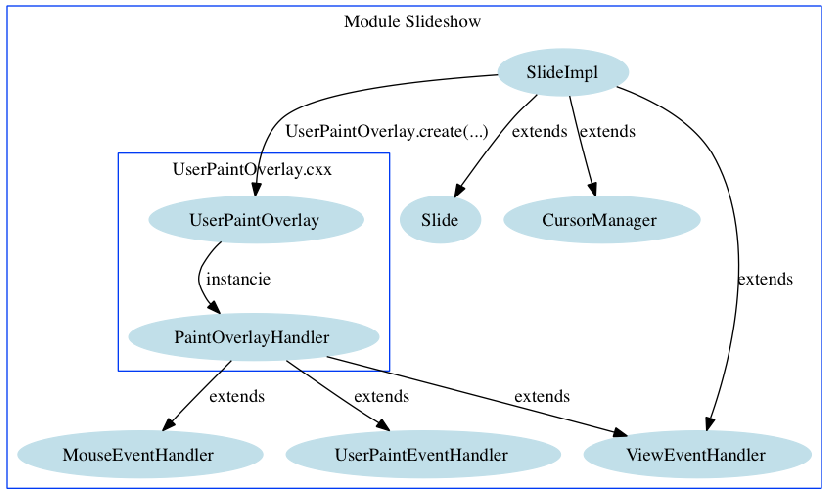
\includegraphics[scale=0.5]{images/Slideshow_module.png}
\caption{The Slideshow module in OOo4Kids}
\end{figure}   

In sd/source/engine, the class slideshowimpl.cxx allows to statically and
dynamically show a presentation. This class also relies on user interaction,
the interface providing means to register some UI event listener. This class
realizes the interface between the previous sd module slideshowimpl class.

We can indeed find the method setProperty, mentioned before. The method
setProperty is merely an interface between UI and the eventmultiplexer. We
indeed can observe links between the two classes:

\begin{lstlisting}[language=C++]
    else if( slideSwitchContextMode && ( CURSOR \paragraph{*slideSwitchContextMode ))
        nCursorShape = awt::SystemPointer::ARROW;
\end{lstlisting}

and a new enum :

\begin{lstlisting}[language=C++]
    enum                                    SlideSwitchContextMode {
                                                CURSOR,
                                                PEN,
                                                ERASER
    };
\end{lstlisting}

used as an optional boolean with Boost\footnote{The Boost C++ Libraries are a
collection of free libraries that extend the functionality of C++.}

\begin{lstlisting}[language=C++]
    //changed for the eraser project
    boost::optional<bool>                    maEraseAllInk;
    boost::optional<SlideSwitchContextMode>  slideSwitchContextMode;
    boost::optional<sal_Int32>               maEraseInk;
    //end changed
\end{lstlisting}

The header of this class is not in the same folder. It can be found in
\emph{slideshow/source/inc/userpainteventhandler.hxx}.


The eventmultiplexer class listens to the XslideShowView and fires events
registered for certain user actions. Other state changes (start and end of
slide) are handled in this class as well.

Therefore, the actions of the menu called by the user are registered here. For
example, for the action « notifySwitchCursorMode » in
\emph{slideshow/source/engine/eventmultiplexer.cxx}

\begin{lstlisting}[language=C++]
bool EventMultiplexer::notifySwitchCursorMode(){
    return mpImpl->maUserPaintEventHandlers.applyAll(
	    boost::mem_fn(&UserPaintEventHandler::switchCursorMode));
}
\end{lstlisting}

Once again, the header is not in the same folder, but in
\emph{slideshow/source/inc/eventmultiplexer.hxx}.

The last class we will be looking at is the userPaintOverlay. This class
registers itself at the EventMultiplexer, listening for mouse clicks and
moves. Therefore, when the mouse is dragged, an annotation is drawn, or
erased, depending which mode is activated. We can find in this class most of
the methods concerning the annotation drawing and erasing. We will not detail
more the methods of this class, since a plain code review is sufficient to
understand most of the concept of the class.


\subsubsection*{Implementing the new functionalities}
\addcontentsline{toc}{subsubsection}{Implementing the new functionalities}

We split the work in 3 parts :

\begin{itemize}

\item the first part was about replacing booleans describing modes by enum
structures. We worked with files found in former reports made by Centrale
Nantes' students. They were very important for us.

\item we started to work on ui features. We added a link in the context menu
and try to link it to functions.

\item we made cursor functions to work (hardest part of our work)
\end{itemize}

\begin{figure}[!h]
\centering
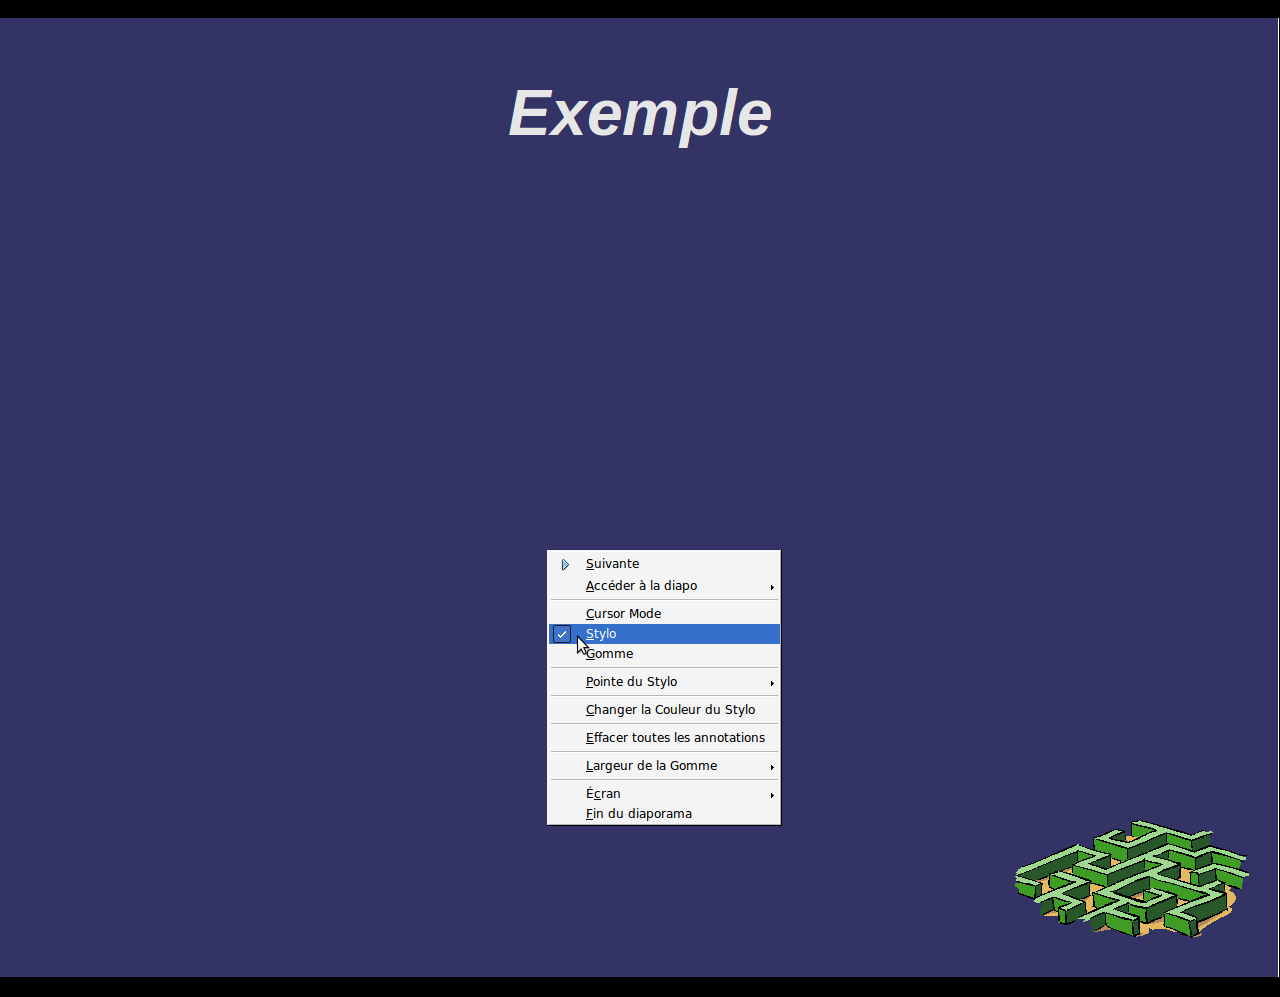
\includegraphics[scale=0.3]{images/screenshot_020.png}
\caption{Screenshot of the context menu (before internationalization)}
\end{figure}

\begin{figure}[!h]
\centering
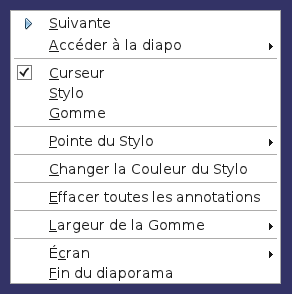
\includegraphics[scale=0.5]{images/Context_menu.png}
\caption{Screenshot of the context menu ready for release}
\end{figure}

\subsubsection*{Code protection}
\addcontentsline{toc}{subsubsection}{Code protection}

Our goal was to develop functionalities in Impress, the slideshow presentation
program. It was very important to protect our code in order to allow a
compilation without compiling our functionalities.

These protections give us the possibility to create versions without Tablet PC
options and the annotations in a presentation and to deliver a repository with
our changes, even if there is problem in our code and our work is not
complete. We used the variable created by former students from École Centrale
de Nantes.

The variable ENABLE\_PRESENTER\_EXTRA\_UI is set when we configure the
compilation with the command ./configure - -enable-presenter-extra-ui

Example with the protection in file
\emph{slideshow/source/engine/slide/userpaintoverlay.hxx}:

\begin{lstlisting}[language=C++]
void SAL_CALL SlideshowImpl::setPenColor( sal_Int32 nColor )
 throw (RuntimeException)
{
	::vos::OGuard aSolarGuard( Application::GetSolarMutex() );
	mnUserPaintColor = nColor;
#ifdef ENABLE_PRESENTER_EXTRA_UI
    slideSwitchToMode = PEN;
	//mbSwitchPenMode = true;
	//mbSwitchEraserMode = !mbSwitchPenMode;
#endif
	if( maPresSettings.mbMouseAsPen )
		setUsePen( sal_True ); // update color
}

#ifdef ENABLE_PRESENTER_EXTRA_UI
// --------------------------------------------------------------------
\end{lstlisting}

And in the makefile :

\begin{verbatim}
.IF "$(ENABLE_PRESENTER_EXTRA_UI)"=="YES"
CDEFS+= -DENABLE_PRESENTER_EXTRA_UI
.ENDIF
\end{verbatim}

Conclusion Protecting our code was important and mandatory to deliver a clean
repository. If we would to have this code integrated to LibreOffice, we will
have to improve this point. This is not so important for OOo4Kids as
ENABLE\_PRESENTER\_EXTRA\_UI is always set to YES.

\subsubsection*{Hotkeys}
\addcontentsline{toc}{subsubsection}{Hotkeys}

We found this in a former report. We wanted to implement hot-keys but we were
having a lack of time. A good starting point for a next patch could be
realising hotkeys for this menu.

\newpage
\rhead{\Large{\textsc{Weekly Description}}}
\fancyfoot[C]{\thepage}
\section*{Weekly Description}
\addcontentsline{toc}{section}{Weekly Description}

\subsection*{Benjamin's notes}
\addcontentsline{toc}{subsection}{Benjamin's notes}

\subsubsection*{From March, 7th 2011, to March, 13th 2011}
\addcontentsline{toc}{subsubsection}{From March, 7th 2011, to March, 13th 2011}

The cursor menu is now complete. Ready for review :-D !

Found my bug with rasqal. I now use --with-system-redland and installed
librdf0-dev on my computer

The bug with PEN activated by default in the slideshow is now closed. It was
due to a else{} not correctly added in
\emph{slideshow/source/engine/slide/userpaintoverlay.cxx}

We are still working on setUsePen() and setUseCursor(). setUseCursor() is
still inefficient.

Moreover, we added the "tick" for the Curseur mode and the menu entry is now
both translated in French and English.

The cursor menu is now displaying an arrow. The only thing that remains is to
have the cursor not acting as a pen or as an eraser. Once our code will be
clean, it will be ready for review.

\subsubsection*{From February, 21th 2011, to February, 28th 2011}
\addcontentsline{toc}{subsubsection}{From February, 21th 2011, to February, 28th 2011}

I am trying to build OOo4Kids on my Debian Sid o my laptop.  It doesn't work :
I have exactly the same issues described here : http://www.pastie.org/1598185

No way to solve this. It is definitely a roadblock.

We are looking for \#ifdef ENABLE\_PRESENTER\_EXTRA\_UI around the code to
find were the pen mode is started...

\subsubsection*{From February, 14th 2011, to February, 20th 2011}
\addcontentsline{toc}{subsubsection}{From February, 14th 2011, to February, 20th 2011}

Clément and I found the eraser bug ! We polished our patch with enum
structures instead of many booleans. The patch has been sent for review. Next
step is to complete our method setUseCursor to have a cursor instead of a pen
during presentation mode.


\subsubsection*{From January, 7th 2011, to February, 13th 2011}
\addcontentsline{toc}{subsubsection}{From January, 7th 2011, to February, 13th 2011}

A bug with the eraser suddenly appears. When clicking on eraser menu, the
eraser icon is loaded but the eraser still have abilities of pen. So it must
be a Boolean issue. Last year, students already had the same issue. We are
re-reading reports to find help.

We are running OOo4Kids through gdb to find how we could remove this bug.

\subsubsection*{From January, 31th 2011, to February, 6th 2011}
\addcontentsline{toc}{subsubsection}{From January, 31th 2011, to February, 6th 2011}

We are working on \emph{sd/source/ui/slideshow/slideshowimpl.cxx/hxx}. We
discovered two classes with the same name (SlideShowImpl and SlideshowImpl)
which are used for Shlideshow drawing mode.

We are deleting some booleans and replacing them with enum structure. (
\emph{mbSwitchPenMode} and \emph{mbSwitchEraserMode} )

A new menu entry has been created (still not internationalized (i18n) /
localized (l10n) yet) in \emph{/sd/source/ui/slideshow/slideshow.src}

Moreover, we added several methods : \emph{virtual void SAL\_CALL
setUseCursor( ::sal\_Bool \_usecursor )} in
\emph{/sd/source/ui/slideshow/slideshow.hxx} for example.

\subsubsection*{From January, 24th 2011, to January, 30th 2011}
\addcontentsline{toc}{subsubsection}{From January, 24th 2011, to January, 30th 2011}

We are adding a new mode, called CM\_CURSOR\_MODE in slideshow.src/cxx

We created a new patch with the enum structure only. We are looking at
\emph{sd/source/ui/slideshow/slideshow.src}. We are doing to implement the new
behavior of the menu.

We also created a Git repository of OOo4Kids to be able to have easy pull/push
between us. We deployed our Git Server on Campus's server which is the
student's server in Centrale Nantes.

We still noticed : userpaintoverlay.cxx should be called
paintoverlayhandler.cxx ? Shall we rename this file ?

\subsubsection*{From January, 17th 2011, to January, 23th 2011}
\addcontentsline{toc}{subsubsection}{From January, 17th 2011, to January, 23th 2011}

On Friday, January 21st, our first patch has been integrated : 08:43 < CIA-65>
OOo4Kids: ericb * r1134 /trunk/slideshow/source/engine/slideshowimpl.cxx:
Applying the patch from Benjamin Vialle and Clement Delafargue. Cleanup in
slideshow. Thanks to them.

We have now two patches of 800 and 1700 lines :-)

We are working on creating an enum type for the pen/eraser/cursor menu. First
thing, search for the right file containing this.

Edit : Ok. Got it : \emph{slideshow/source/engine/slide/userpaintoverlay.cxx}

We cleaned \emph{slideshow/source/engine/slide/userpaintoverlay.cxx} and
\emph{slideshow/source/engine/slide/userpaintoverlay.hxx}.  We noticed :
userpaintoverlay.cxx should be called paintoverlayhandler.cxx ? Shall we
rename this file ?

We have re-indented, removed trailing white paces and tabs from
\emph{slideshow/source/engine/slideshowimpl.cxx}

By cleaning, are we supposed to create a header (.h) file containing
definition of the class ?

Summary from former projects have been written to the Centrale Nantes wiki's
page (see [[Applications/CentraleNantes|Centrale Nantes]]).

We added our Specification Book on [[Applications/CentraleNantes|Centrale
Nantes - Planned Work (2011)]].

\subsubsection*{From January, 10th 2011, to January, 16th 2011}
\addcontentsline{toc}{subsubsection}{From January, 10th 2011, to January, 16th 2011}

Clément and I started to write the Specification Book.

We worked on the Gentoo part of the setup page.

We decided to plan a meeting each tuesday at 9PM, with Éric Bachard.

We will have to talk about the OpenOffice.org former way to build OOo on
Gentoo (see
\url{http://wiki.services.openoffice.org/wiki/Gentoo\_build\_instructions} ) I
don't agree with their way to proceed. According to Gentoo's ebuild for OOo,
we DO NOT need rpm to be installed. And it is obvious :-)

\subsubsection*{From January, 3rd 2011, to January, 9th 2011}
\addcontentsline{toc}{subsubsection}{From January, 3rd 2011, to January, 9th 2011}

The compilation was complete, but the OoImpress module crashed on stratup. A
segfault with hunspell.  The compilation with \emph{'--with-system-hunspell'}
solved this issue.


%Conclusion sur une page non numérotée et intégrée à la table des matières.
\newpage
\rhead{\Large{\textsc{Conclusion}}}
\section*{Conclusion}
\addcontentsline{toc}{section}{Conclusion}

It was a very interesting work to discover OpenOffice.org source code.  The
codebase is really big, and some parts are getting quite old. It took us some
time and effort to understand how it works. There are many layers which
communicate \emph{via} different means. Is was the second time we worked on 
FOSS\footnote{Free Open Source Software}, but this time the project was orders
of magnitude older and bigger. In any case, the strength and the power of the
community is really important.

Working with Éric \textsc{Bachard} was very helpful. We learned how to
understand the code in good conditions. He gave us good hints and starting
points when chasing bugs or starting to implement features.

At the FOSDEM in february 2011, we had the opportunity to talked to
OpenOffice.org developpers (Norvegian ones !). We saw presentations from the
LibreOffice project (with Thorsten \textsc{Berhens})

A good end could be the integration of our patch in other OpenOffice.org4Kids
forks or parents, like OpenOffice.org, LibreOffice or Go-oo.

We are very thankful to Éric \textsc{Bachard} for his help.

\newpage
\rhead{\Large{\textsc{Images}}}
\addcontentsline{toc}{section}{List of images}
\listoffigures

\newpage
\rhead{\Large{\textsc{Appendix}}}
\section*{Appendix}
\addcontentsline{toc}{section}{Appendix}

\begin{figure}[h!]
    \centering
	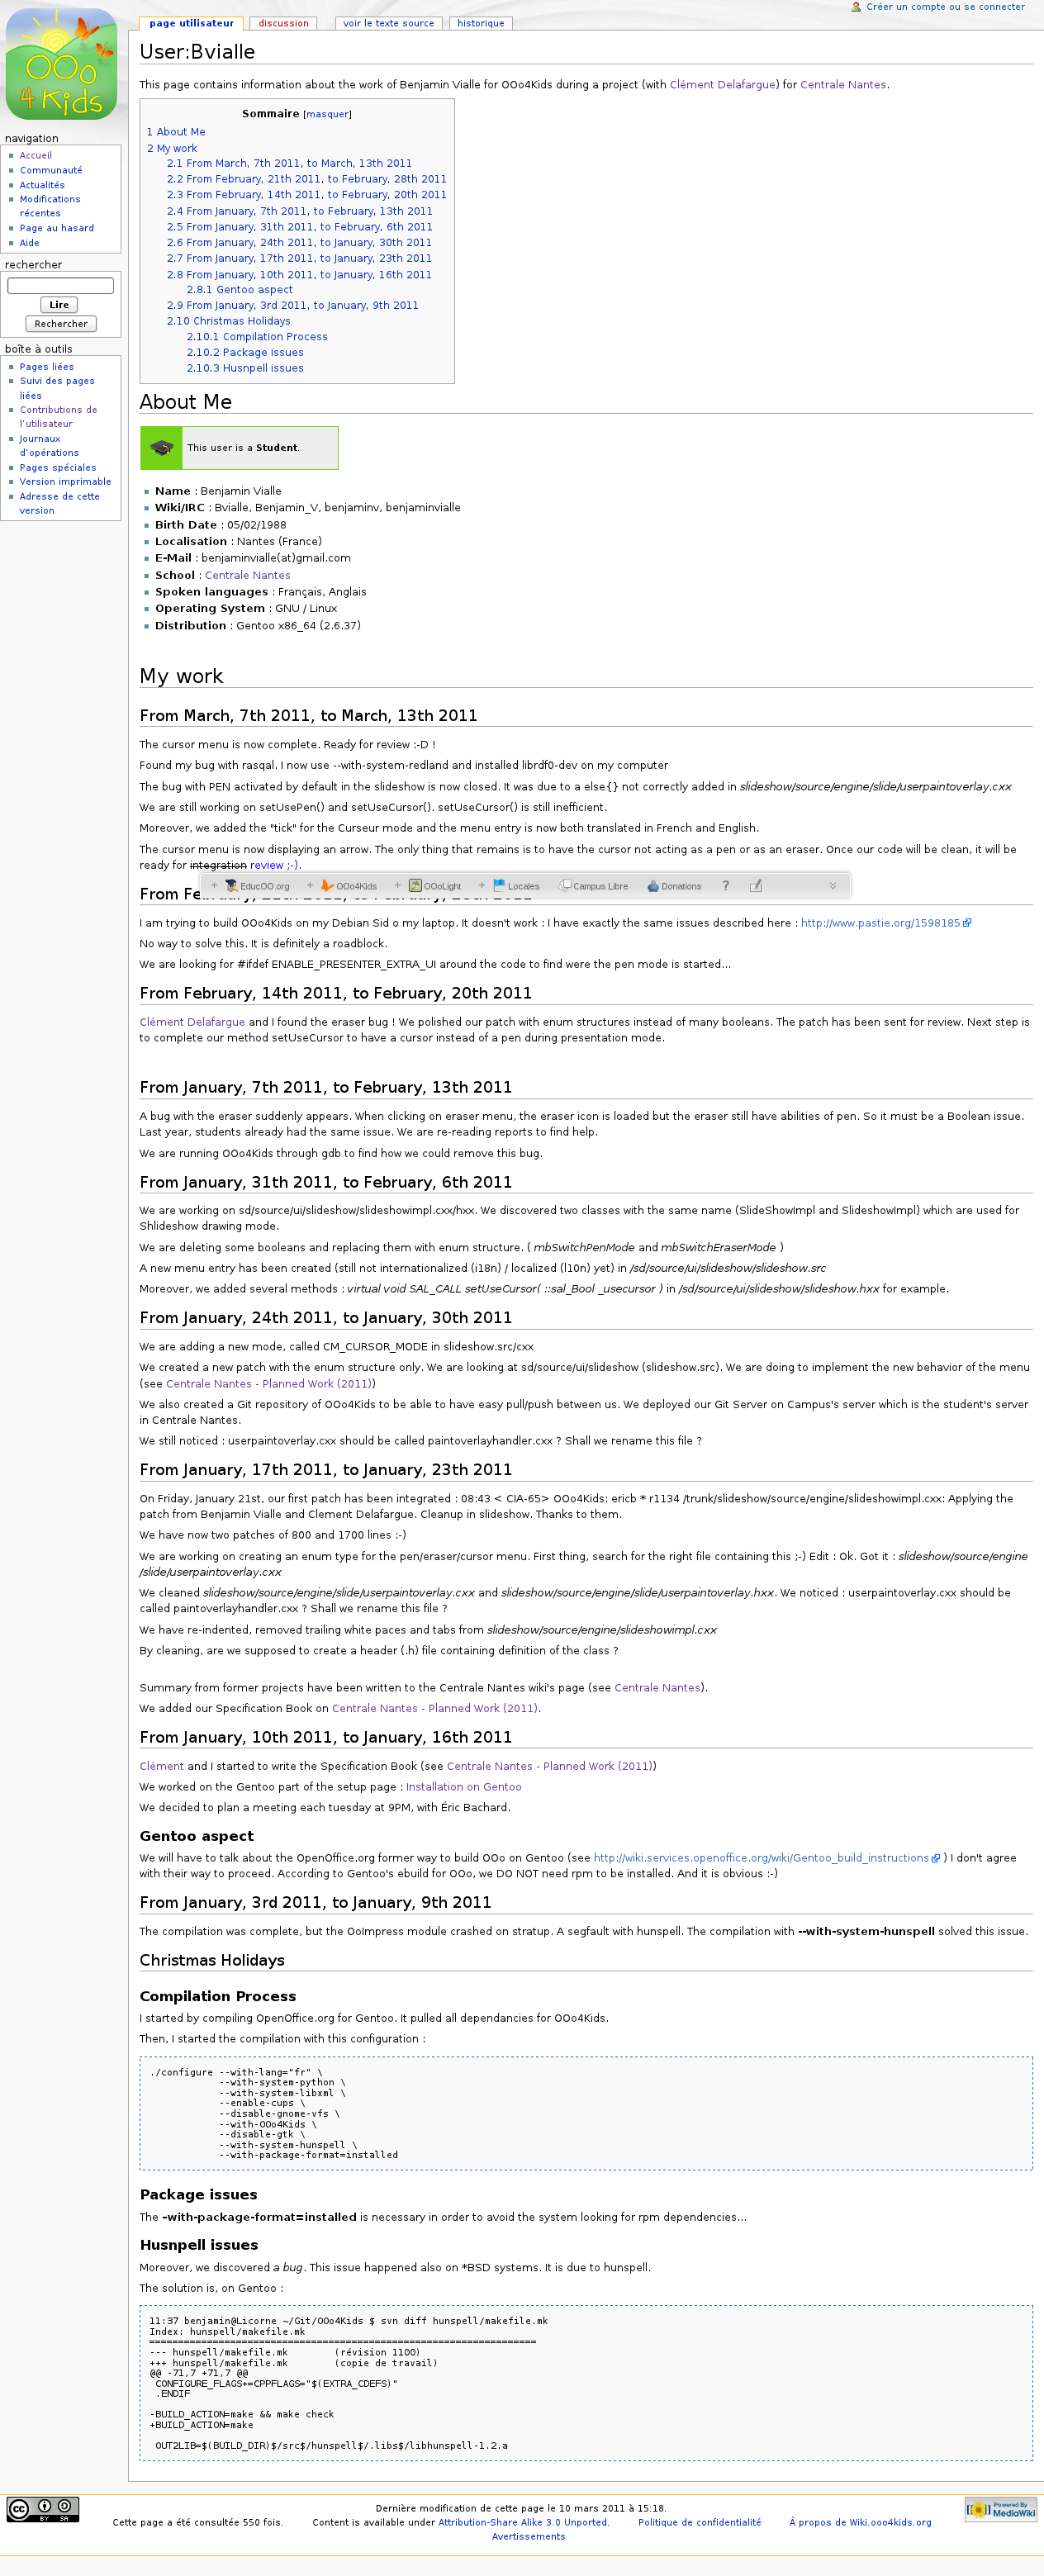
\includegraphics[scale=0.2]{images/OOo4Kids_bvialle.png}
	\caption{Benjamin's page on OOo4Kids'wiki}
\end{figure}



\end{document}
